\documentclass[10pt]{article}
\usepackage{amsmath, amssymb, amsthm}
\usepackage[top=2cm, left = 2cm, right = 2cm, bottom = 3cm]{geometry}
\usepackage[pdftex]{graphicx}
\usepackage{asymptote}
\usepackage{tikz}
\usepackage{multicol}
\usepackage{fancyhdr}
\newcommand{\N}{\mathbb{N}}
\pagestyle{fancy}
\rhead{}
\chead{\includegraphics[scale=0.1]{../CMIMC-header-2018.png}}
\lhead{}
\setlength{\headheight}{43pt}
\rfoot{}
\cfoot{}
\lfoot{}
\newcommand{\proposed}[1]
{
\vspace{5pt}
\noindent\textit{Proposed by #1}
}
\newcommand{\solution}
{
\vspace{5pt}
\noindent\textit{Solution.}\qquad
}
\begin{document}\thispagestyle{empty}
\begin{center}

\vspace*{40pt}

\includegraphics[scale=0.2]{../CMIMC-header-2018.png}

\includegraphics[scale=0.3]{CS-header.png}

\vspace{1.4in}

\includegraphics[scale=0.20]{Instruction-Header.png}
\noindent\rule{15.7cm}{2pt}
\end{center}

\vspace{10pt}

\input{input/test-instructions}

\vspace{0.7in}

\begin{center}
\includegraphics[scale=0.15]{../sponsor-footer.png}
\end{center}
\newpage

\begin{center}
\huge\textbf{Computer Science}\normalsize

\vspace{3pt}
\end{center}

\begin{enumerate}
%\item Find all pairs of integer constants $(b, d)$ such that \[(3\log(t) + bt)(8\log(t) + dt) - bdt^2 + (95+ bd)t\log(t)\] is $o(t)$

\item Consider the following two vertex-weighted graphs, and denote them as having vertex sets $V=\{v_1,v_2,\ldots,v_6\}$ and $W=\{w_1,w_2,\ldots,w_6\}$, respectively (numbered in the same direction and way). The weights in the second graph are such that for all $1\le i\le 6$, the weight of $w_i$ is the sum of the weights of the neighbors of $v_i$.
Determine the sum of the weights of the original graph.

\begin{center}
\begin{multicols}{2}

\begin{tikzpicture}[scale=0.7]

  \def \n {6}
  \def \radius {3cm}
  \def \margin {8} % margin in angles, depends on the radius
  
  \foreach \s in {1,...,\n}
  {
    \node[draw, circle, inner sep=0.25cm] (N-\s) at ({360 - 360/\n * (\s - 1) + 90}:\radius) {$v_\s$};
  }

%   \foreach \number in {1,...,\na}{
%     \foreach \numbera in {\number,...,\n}{
%         \path (N-\number) edge[] (N-\numbera)  edge[] (N-\numbera);
%     }
%   }
  \path (N-1) edge[] (N-5) edge[] (N-5);
  \path (N-1) edge[] (N-6) edge[] (N-6);
  \path (N-2) edge[] (N-3) edge[] (N-3);
  \path (N-2) edge[] (N-4) edge[] (N-4);
  \path (N-2) edge[] (N-6) edge[] (N-6);
  \path (N-3) edge[] (N-4) edge[] (N-4);
  \path (N-3) edge[] (N-5) edge[] (N-5);
  \path (N-5) edge[] (N-6) edge[] (N-6);

\end{tikzpicture}

%(v1,v2,v3,v4,v5,v6) = (2, 3, 4, 6, 8, 9)
%w1 = v5+v6 = 8+9 = 17
%w2 = v3+v4+v6 = 4+6+9 = 19
%w3 = v2+v4+v5 = 3+6+8 = 17
%w4 = v2+v3 = 3+4 = 7
%w5 = v1+v3+v6 = 2+4+9 = 15
%w6 = v1+v2+v5 = 2+3+8 = 13
\begin{tikzpicture}[scale=0.7]
  \def \n {6}
  \def \radius {3cm}
  \def \margin {8} % margin in angles, depends on the radius
  
%   \foreach \s in {1,...,\n}
%   {
%     \node[draw, circle, inner sep=0.25cm] (N-\s) at ({360 - 360/\n * (\s - 1) + 90}:\radius) {$v_\s$};
%   }

  \node[draw, circle, inner sep=0.25cm] (N-1) at ({360 - 360/\n * (1 - 1) + 90}:\radius) {17};
  
  \node[draw, circle, inner sep=0.25cm] (N-2) at ({360 - 360/\n * (2 - 1) + 90}:\radius) {19};
  
  \node[draw, circle, inner sep=0.25cm] (N-3) at ({360 - 360/\n * (3 - 1) + 90}:\radius) {17};
  
  \node[draw, circle, inner sep=0.25cm] (N-4) at ({360 - 360/\n * (4 - 1) + 90}:\radius) {7};
  
  \node[draw, circle, inner sep=0.25cm] (N-5) at ({360 - 360/\n * (5 - 1) + 90}:\radius) {15};
  
  \node[draw, circle, inner sep=0.25cm] (N-6) at ({360 - 360/\n * (6 - 1) + 90}:\radius) {13};

%   \foreach \number in {1,...,\na}{
%     \foreach \numbera in {\number,...,\n}{
%         \path (N-\number) edge[] (N-\numbera)  edge[] (N-\numbera);
%     }
%   }
  \path (N-1) edge[] (N-5) edge[] (N-5);
  \path (N-1) edge[] (N-6) edge[] (N-6);
  \path (N-2) edge[] (N-3) edge[] (N-3);
  \path (N-2) edge[] (N-4) edge[] (N-4);
  \path (N-2) edge[] (N-6) edge[] (N-6);
  \path (N-3) edge[] (N-4) edge[] (N-4);
  \path (N-3) edge[] (N-5) edge[] (N-5);
  \path (N-5) edge[] (N-6) edge[] (N-6);
  
\end{tikzpicture}

\end{multicols}

\end{center}

% also not that good
\item Consider the natural implementation of computing Fibonacci numbers:

\begin{tabular}{l}
1: \textbf{FUNCTION} $\text{FIB}(n)$: \\
2:$\qquad$ \textbf{IF} $n = 0$ \textbf{OR} $n = 1$ \textbf{RETURN} 1 \\
3:$\qquad$ \textbf{RETURN} $\text{FIB}(n-1) + \text{FIB}(n-2)$
\end{tabular}

When $\text{FIB}(10)$ is evaluated, how many recursive calls to $\text{FIB}$ occur?

\item You are given the existence of an unsorted sequence $a_1,\ldots, a_5$ of five distinct real numbers.  The Erdos-Szekeres theorem states that there exists a subsequence of length $3$ which is either strictly increasing or strictly decreasing.  You do not have access to the $a_i$, but you do have an oracle which, when given two indexes $1\leq i < j\leq 5$, will tell you whether $a_i < a_j$ or $a_i > a_j$.  What is the minimum number of calls to the oracle needed in order to identify an ordered triple of integers $(r,s,t)$ such that $a_r,a_s,a_t$ is one such sequence?

%Answer: 4. It is easy to see that three does not work; one can consider all possible sets of calls and for each one construct an ordering of the a_i which prevents determining a desired sequence.  Now we exhibit a sequence of four calls which works.  First call the oracle on (2,3), (3,4), and (2,4).  This allows us to determine a total ordering of the #s a2, a3, a4.  We now case on which one of these is the median.  If it's a3, (2,3,4) works.  Otherwise, WLOG a3 < a2 < a4.  Now call (1,2).  Then *if a1 < a2, then (1,2,4) works; *if a1 > a2, then (1,2,3) works.  We're done.

\item Consider the grid of numbers shown below.

\begin{center}
\begin{verbatim}
                                      20 01 96 56 16
                                      37 48 38 64 60
                                      96 97 42 20 98
                                      35 64 96 40 71
                                      50 58 90 16 89
\end{verbatim}
\end{center}

Among all paths that start on the top row, move only left, right, and down, and end on the bottom row, what is the minimum sum of their entries?

\item An \textit{access pattern} $\pi$ is a permutation of $\{1,2,\dots,50\}$ describing the order in which some $50$ memory addresses are accessed. We define the \textit{locality} of $\pi$ to be how much the program jumps around the memory, or numerically, \[\sum_{i=2}^{50}\left\lvert\pi(i)-\pi(i-1)\right\rvert.\] If $\pi$ is a uniformly randomly chosen access pattern, what is the expected value of its locality?

%\item The \emph{distance} between two vertices in a connected graph is defined to be the length of the shortest path between them. How many graphs with the vertex set $\{0,1,2,\dots,6\}$ satisfy the following property: there are $3$ vertices of distance $1$ away from vertex $0$, $2$ of distance $2$ away, and $1$ of distance $3$ away?

\item For integer $n\geq 2$ and real $0\leq p\leq 1$, define $\mathcal{W}_{n,p}$ to be the complete weighted undirected random graph with vertex set $\{1,2,\ldots,n\}$: the edge $(i,j)$ will have weight $\min(i,j)$ with probability $p$ and weight $\max(i,j)$ otherwise. Let $\mathcal{L}_{n,p}$ denote the total weight of the minimum spanning tree of $\mathcal{W}_{n,p}$. Find the largest integer less than the expected value of $\mathcal{L}_{2018,1/2}$.


\item I give you a function \textbf{rand} that returns a number chosen uniformly at random from $[0,T]$ for some number $T$ that you don't know. Your task is to approximate $T$. You do this by calling \textbf{rand} $100$ times, recording the results as $X_1,X_2,\dots,X_{100}$, and guessing \[\hat{T}=\alpha\cdot\max\{X_1,X_2,\dots,X_{100}\}\] for some $\alpha$. Which value of $\alpha$ ensures that $\mathbb{E}[\hat{T}]=T$?

\item We consider a simple model for balanced parenthesis checking. Let $\mathcal R=\{\texttt{(())}\rightarrow \texttt{A},\texttt{(A)}\rightarrow\texttt{A},\texttt{AA}\rightarrow\texttt{A}\}$ be a set of rules for phrase reduction. Ideally, any given phrase is balanced if and only if the model is able to reduce the phrase to \texttt{A} by some arbitrary sequence of rule applications. For example, to show \texttt{((()))} is balanced we can perform the following sequence of reductions.
\[\texttt{((()))}\rightarrow\texttt{(A)}\rightarrow\texttt{A}\qquad \checkmark\]
Unfortunately, the above set of rules $\mathcal R$ is not complete, since there exist parenthetical phrases which are balanced but which are not balanced according to $\mathcal R$.  Determine the number of such phrases of length $14$. %; find the number of balanced parenthetical phrases of length $14$ for which $\mathcal R$ \textbf{is insufficient} to show that they are balanced.

%\item Consider a connected graph $G$ with vertex set $\{0,1,2,\dots,n\}$. Suppose there exist $a_1$ vertices of distance $1$ away from vertex $0$, $a_2$ vertices of distance $2$ away from vertex $0$, $\dots$, $a_m$ vertices of distance $m$ away from vertex $0$ (where $a_1+\dots+a_m=n$). How many such graphs satisfy this property?

\item Consider the following modified algorithm for binary search, which we will call \textit{weighted binary search}:

\begin{tabular}{l}
01: \textbf{FUNCTION} SEARCH($L$, value) \\
02:$\qquad$  hi $\leftarrow$ $\operatorname{len}(L) - 1$ \\
03:$\qquad$  lo $\leftarrow$ 0 \\
04:$\qquad$  \textbf{WHILE} hi $\geq$ lo \\
05:$\qquad\qquad$ guess $\leftarrow$ $\lfloor w \cdot\text{lo} + (1-w) \cdot \text{hi}\rfloor$ \\
06:$\qquad\qquad$ mid $\leftarrow$ $L[\text{guess}]$ \\
07:$\qquad\qquad$ \textbf{IF} mid $> \text{value}$ \\
08: $\qquad\qquad\qquad$ hi $\leftarrow$ $\text{guess} - 1$ \\
09: $\qquad\qquad$ \textbf{ELSE IF} mid $< \text{value}$ \\
10: $\qquad\qquad\qquad$ lo $\leftarrow$ $\text{guess} + 1$ \\
11: $\qquad\qquad$ \textbf{ELSE} \\
12: $\qquad\qquad\qquad$ \textbf{RETURN} guess \\
13:$\qquad$ \textbf{RETURN} -1 (not found) 
\end{tabular}\\

Assume $L$ is a list of the integers $\{1,2,\ldots,100\}$, in that order. Further assume that accessing the $k$th index of $L$ costs $k+1$ tokens (e.g. $L[0]$ costs $1$ token). Let $S$ be the set of all $w\in[\tfrac12,1)$ which minimize the average cost when \texttt{value} is an integer selected at random in the range $[1,50]$. Given that $S=\left(x,\tfrac {74}{99}\right]$, determine $x$.

\item Consider an undirected, connected graph $G$ with vertex set $\{v_1,v_2,\ldots, v_6\}$.  Starting at the vertex $v_1$, an ant uses a DFS algorithm to traverse through $G$ under the condition that if there are multiple unvisited neighbors of some vertex, the ant chooses the $v_i$ with smallest $i$.  How many possible graphs $G$ are there satisfying the following property: for each $1\leq i\leq 6$, the vertex $v_i$ is the $i^{\text{th}}$ new vertex the ant traverses?

\end{enumerate}

\end{document}